%----------------------------------------------------------------------------------------
%	PACKAGES AND DOCUMENT CONFIGURATIONS
%----------------------------------------------------------------------------------------
\documentclass{article}
%\documentclass[tikz, border=2mm]{standalone}

\usepackage{siunitx} % Provides the \SI{}{} and \si{} command for typesetting SI units
\usepackage{graphicx} % Required for the inclusion of images
\usepackage{natbib} % Required to change bibliography style to APA
\usepackage{amsmath} % Required for some math elements 
\setlength\parindent{12pt} % Removes all indentation from paragraphs
%\usepackage{times} % Uncomment to use the Times New Roman font

\usepackage[export]{adjustbox}

\usepackage[utf8]{inputenc} % Język polski
\usepackage{polski}
\usepackage[polish]{babel}

\usepackage[top=1in, bottom=1.25in, left=1.25in, right=1.25in]{geometry} % Marginesy
\usepackage{listings} % Kod programu
\usepackage{indentfirst} % Wcięcie przy pomocy \par
\usepackage{multicol} % Kilka kolumn dla itemize
\usepackage[table,xcdraw]{xcolor} % Dla tabel
\usepackage{float} % Blokowanie tabeli przed przemieszczeniem
%\usepackage{karnaugh-map} % Karnaugh

%\renewcommand{\labelenumi}{\alph{enumi}.} % Zamienia litery w enumerate na a, b, c, ...


\usepackage{multirow}
%----------------------------------------------------------------------------------------
%	DOCUMENT INFORMATION
%----------------------------------------------------------------------------------------

\title{Technologie Sieciowe 2 - Projekt \\ \textit{Projekt sieci lokalnej dla biura projektowego}} % Title

\author{Jan \textsc{Pajdak} \\ Wojciech \textsc{Słowiński}} % Author name

\date{12.11.2017} % Date for the report
%\date{\today} % Date for the report

\begin{document}

\maketitle % Insert the title, author and date

\begin{center}
\begin{tabular}{l r}
%Data: <data> \\ % Date the experiment was performed
%Prowadzący: & Mgr inż. Jan Paweł II % Instructor/supervisor
Prowadzący: & Dr inż. Przemysław Ryba \\
Termin zajęć: & Wtorek 9:15 TP \\
Grupa: & 3 
%Prowadzący: & Dr inż. Tomasz Babczyński
%Prowadzący: & Dr inż. Tomasz Walkowiak
%Prowadzący: & Dr inż. Jarosław Sugier
%Prowadzący: & Mgr inż. Szymon Datko
\end{tabular}
\end{center}

\tableofcontents % Spis treści

% If you wish to include an abstract, uncomment the lines below
% \begin{abstract}
% Abstract text
% \end{abstract}

%----------------------------------------------------------------------------------------
%	SECTION 0
%----------------------------------------------------------------------------------------

%\begin{multicols}{2}
%	\begin{itemize}
%		\item 
%	\end{itemize}
%\end{multicols}

%\newpage
%\section{Tytuł}} 
%\subsection{Tytuł}
%\par Tekst

%\begin{itemize}
%	\item\textit{Tekst} - Opis
%\end{itemize}

%\begin{enumerate}
%	\item Opis
%\end{enumerate}

%\begin{center}
%	\includegraphics[scale=0.6, center]{nazwa_pliku}
%\end{center}

%\begin{lstlisting}[basicstyle=\small]
%	kod programu;
%\end{lstlisting}

%----------------------------------------------------------------------------------------
%	SECTION 1
%----------------------------------------------------------------------------------------
% Scharakteryzować profil działania przedsiębiorstwa/instytucji. Opisać cel projektu.
% Dodatkowe założenia i odpowiedzi na często zadawane pytania
% - instalacje dostawców usług internetowych zostaną doprowadzone do MDF
% - serwery mają zostać zainstalowane w szafach teleinformatycznych (decyzja w których należy do projektantów)
% - każdy z serwerów wyposażony jest w dwa porty 1Gb/s (RJ-45)
\newpage
\section{Wstęp}
\subsection{Cel projektu}
\par Celem projektu jest zaprojektowanie sieci komputerowej dla przedsiębiorstwa. Budynki przedsiębiorstwa są wyposażone w okablowanie strukturalne, szafy teleinformatyczne oraz urządzenia końcowe. Zakres projektu obejmuje:
\begin{enumerate}
	\item Projekt logiczny sieci.
	\item Projekt VLAN.
	\item Wybór oraz konfigurację urządzeń sieciowych.
\end{enumerate}
\par W zakres projektu wchodzi także wybór dostawcy internetowego.

\subsection{Profil działania przedsiębiorstwa}
\par Zleceniodawcą jest biuro projektowe zatrudniające 497 pracowników; każdy z nich posiada własne stanowisko komputerowe podłączone do sieci. Przedsiębiorstwo znajduje się w dwóch budynkach oddalonych od siebie o 379 metrów; pierwszy z nich ma dwa piętra a drugi trzy. Budynki są połączone przy użyciu technologii optycznej wielomodowej.
\begin{center}
	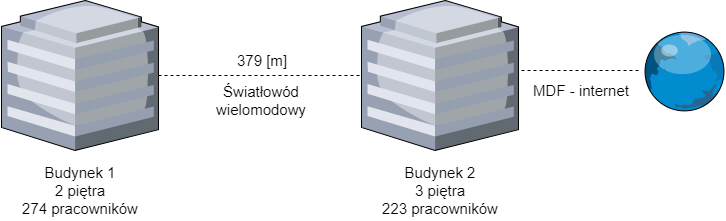
\includegraphics[scale=0.55, center]{buildings_b}
\end{center}

%----------------------------------------------------------------------------------------
%	SECTION 2
%----------------------------------------------------------------------------------------
% Zamieścić i omówić dane uzyskane od Prowadzącego.
\newpage
\section{Inwentaryzacja zasobów}
\par Tabele określające ilość użytkowników danej grupy zostały umieszczone poniżej. Każdy rodzaj użytkownika ma inne wymagania (określone w sekcji 3.1). Dodatkowo niewielka ilość użytkowników będzie pracowała przy użyciu sieci WiFi.

\begin{table}[H]
	\centering
	\caption{Liczba użytkowników}
	%\label{my-label}
\begin{tabular}{|l|c|c|c|c|c|}
	\hline
	\textbf{Budynek}                                                                   & \multicolumn{2}{c|}{1}      & \multicolumn{3}{c|}{2}                  \\ \hline
	\textbf{Piętro}                                                                    & 1            & 2            & 1           & 2           & 3           \\ \hline
	\textbf{Konstruktorzy}                                                             & 41           & 51           & 12          & 50          & 0           \\ \hline
	\textbf{Architekci}                                                                & 48           & 54           & 43          & 20          & 49          \\ \hline
	\textbf{Projektanci}                                                               & 33           & 17           & 18          & 2           & 8           \\ \hline
	\textbf{Zarząd}                                                                    & 6            & 24           & 1           & 8           & 12          \\ \hline
	\textbf{Wszyscy pracownicy}                                                        & \textbf{128} & \textbf{146} & \textbf{74} & \textbf{80} & \textbf{69} \\ \hline
	\textbf{Liczba drukarek}                                                           & 2            & 1            & 3           & 2           & 2           \\ \hline
	\textbf{\begin{tabular}[c]{@{}l@{}}Liczba punktów\\ dostępowych WiFi\end{tabular}} & 3            & 0            & 0           & 0           & 2           \\ \hline
	\textbf{\begin{tabular}[c]{@{}l@{}}Liczba urządzeń\\ bezprzewodowych\end{tabular}} & 17           & 0            & 0           & 0           & 4           \\ \hline
\end{tabular}
\end{table}

\begin{table}[H]
	\centering
	\caption{Punkty dystrybucyjne}
	%\label{my-label}
\begin{tabular}{lll}
	\hline
	\multicolumn{1}{|c|}{\textbf{Oznaczenie}} & \multicolumn{1}{c|}{Lokalizacja} & \multicolumn{1}{c|}{\begin{tabular}[c]{@{}c@{}}Podłączone \\ punkty abonenckie\end{tabular}} \\ \hline
	\multicolumn{1}{|l|}{\textbf{MDF}}        & \multicolumn{1}{l|}{B2-P3}       & \multicolumn{1}{l|}{B2-P3}                                                                   \\ \hline
	\multicolumn{1}{|l|}{\textbf{IDF1}}       & \multicolumn{1}{l|}{B2-P2}       & \multicolumn{1}{l|}{B2-P1/2}                                                                 \\ \hline
	\multicolumn{1}{|l|}{\textbf{IDF2}}       & \multicolumn{1}{l|}{B1-P2}       & \multicolumn{1}{l|}{B1}                                                                      \\ \hline
	\multicolumn{3}{c}{\textit{Przykład: B2-P3: Budynek 2, Piętro 3}}                                                                                                          
\end{tabular}
\end{table}

%----------------------------------------------------------------------------------------
%	SECTION 3
%----------------------------------------------------------------------------------------
% Obliczyć (na podstawie danych od Prowadzącego) i przedstawić oszacowanie transferu danych w kluczowych punktach sieci: łączach szkieletowych 
% (w tym pomiędzy budynkami), łączach do serwerów, łączu do Internetu (w obu kierunkach), itd. Należy zamieścić kompletne obliczenia (a nie same wyniki końcowe).
% Przedstawić pozostałe wymagania, w tym dotyczące bezpieczeństwa i niezawodności sieci.
\newpage
\section{Analiza potrzeb użytkowników}

\subsection{Wymagania przedsiębiorstwa}
\par Przedsiębiorstwo generuje następujący ruch w sieci lokalnej:
\begin{table}[H]
	\centering
	\caption{Wymagania dotyczące przepływów między pracownikami a serwerami}
	%\label{my-label}
\begin{tabular}{|l|c|c|c|c|c|c|c|c|}
	\hline
	\multicolumn{1}{|c|}{\textbf{\begin{tabular}[c]{@{}c@{}}Grupa robocza\\ lub serwer\end{tabular}}} & \multicolumn{2}{c|}{Serwer 1} & \multicolumn{2}{c|}{Serwer 2} & \multicolumn{2}{c|}{Serwer 3} & \multicolumn{2}{c|}{Drukarka} \\ \hline
	\textbf{Prędkość {[}kb/s{]}}                                                                      & Down           & Up           & Down           & Up           & Down           & Up           & Down           & Up           \\ \hline
	\textbf{Konstruktorzy}                                                                            & 500            & 650          & 0              & 0            & 250            & 950          & 10             & 100          \\ \hline
	\textbf{Architekci}                                                                               & 150            & 500          & 650            & 150          & 500            & 500          & 10             & 110          \\ \hline
	\textbf{Projektanci}                                                                              & 0              & 0            & 650            & 500          & 200            & 450          & 10             & 100          \\ \hline
	\textbf{Zarząd}                                                                                   & 0              & 0            & 0              & 0            & 50             & 400          & 10             & 180          \\ \hline
	\textbf{WiFi}                                                                                     & 100            & 150          & 100            & 250          & 200            & 150          & 10             & 120          \\ \hline
\end{tabular}
\end{table}

\begin{table}[H]
	\centering
	\caption{Wymagania dotyczące przepływów generowanych przez aplikacje użytkownika}
	%\label{my-label}
\begin{tabular}{|l|c|c|c|c|c|c|c|c|}
	\hline
	\multicolumn{1}{|c|}{\textbf{\begin{tabular}[c]{@{}c@{}}Grupa robocza\\ lub serwer\end{tabular}}} & \multicolumn{2}{c|}{Przeglądarka} & \multicolumn{2}{c|}{Wideokonferencja} & \multicolumn{2}{c|}{VoIP} & \multicolumn{2}{c|}{Klient FTP} \\ \hline
	\textbf{Prędkość {[}kb/s{]}}                                                                      & Down             & Up             & Down               & Up               & Down         & Up         & Down            & Up            \\ \hline
	\textbf{Konstruktorzy}                                                                            & 0                & 0              & 40                 & 40               & 0            & 0          & 0               & 0             \\ \hline
	\textbf{Architekci}                                                                               & 0                & 0              & 0                  & 0                & 20           & 20         & 57              & 12            \\ \hline
	\textbf{Projektanci}                                                                              & 67               & 10             & 0                  & 0                & 20           & 20         & 72              & 10            \\ \hline
	\textbf{Zarząd}                                                                                   & 66               & 10             & 40                 & 40               & 20           & 20         & 63              & 20            \\ \hline
	\textbf{WiFi}                                                                                     & 18               & 10             & 0                  & 0                & 20           & 20         & 57              & 18            \\ \hline
\end{tabular}
\end{table}

\par Prognoza ruchu między serwerami internetowymi a Internetem została zawarta poniżej. Druga i trzecia kolumna zawierają prędkość transferu (w kb/s) przypadającą na jedną sesję.
\begin{table}[H]
	\centering
	\caption{Prognozowany ruch do Internetu z posiadanych przez firmę serwerów internetowych}
	%\label{my-label}
	\begin{tabular}{|l|c|c|c|}
		\hline
		\multicolumn{1}{|c|}{\textbf{Serwery internetowe}} & Do Internetu & Z Internetu & \begin{tabular}[c]{@{}c@{}}Liczba jednoczesnych\\ sesji\end{tabular} \\ \hline
		\textbf{Serwer WWW}                                & 140          & 35          & 48                                                                   \\ \hline
		\textbf{Serwer FTP}                                & 380          & 70          & 16                                                                   \\ \hline
	\end{tabular}
\end{table}

\newpage
\subsection{Obliczenia}
\par Na podstawie wcześniej wymienionych wymagań można obliczyć przepływ generowany przez pracowników łączących się z serwerami (lub drukarkami) oraz przez aplikacje uruchamiane na komputerach pracowników.
\subsubsection{Przepływ między pracownikami a serwerami}
\begin{table}[H]
	\centering
	\caption{Przepływ między pracownikami a serwerami w Budynku 1}
	%\label{my-label}
\begin{tabular}{|l|c|c|c|c|c|c|c|c|}
	\hline
	\multicolumn{1}{|c|}{\textbf{\begin{tabular}[c]{@{}c@{}}Grupa robocza\\ lub serwer\end{tabular}}} & \multicolumn{2}{c|}{Serwer 1} & \multicolumn{2}{c|}{Serwer 2} & \multicolumn{2}{c|}{Serwer 3} & \multicolumn{2}{c|}{Drukarka} \\ \hline
	\textbf{Prędkość {[}kb/s{]}}                                                                      & Down          & Up            & Down           & Up           & Down          & Up            & Down          & Down          \\ \hline
	\textbf{Konstruktorzy}                                                                            & 46000         & 59800         & 0              & 0            & 23000         & 87400         & 920           & 9200          \\ \hline
	\textbf{Architekci}                                                                               & 15300         & 51000         & 66300          & 15300        & 51000         & 51000         & 1020          & 11220         \\ \hline
	\textbf{Projektanci}                                                                              & 0             & 0             & 32500          & 25000        & 10000         & 22500         & 500           & 5000          \\ \hline
	\textbf{Zarząd}                                                                                   & 0             & 0             & 0              & 0            & 1500          & 14000         & 300           & 5400          \\ \hline
	\textbf{WiFi}                                                                                     & 1700          & 2550          & 1700           & 4250         & 3400          & 2550          & 170           & 2040          \\ \hline
	\textbf{Suma {[}kb/s{]}}                                                                          & 63000         & 11350         & 100500         & 4450         & 88900         & 175450        & 2970          & 32860         \\ \hline
	\textbf{Suma {[}Mb/s{]}}                                                                          & 63            & 11.35         & 100.5          & 4.45         & 88.9          & 175.45        & 2.97          & 32.86         \\ \hline
	\textbf{Suma Down {[}Mb/s{]}}                                                                     & \multicolumn{8}{c|}{\textbf{63 + 100.5 + 88.9 + 2.97 = 255.37}}                                                               \\ \hline
	\textbf{Suma Up {[}Mb/s{]}}                                                                       & \multicolumn{8}{c|}{\textbf{11.35 + 4.45 + 175.45 + 32.86 = 224.11}}                                                          \\ \hline
\end{tabular}
\end{table}
\par Przykładowe obliczenia:
\begin{enumerate}
	\item  $ rozmiar \ grupy \ roboczej \ * \ wymagania \ danej \ grupy \ roboczej = ruch \ grupy \ roboczej $ 
	\\ W Budynku 1 pracuje 92 konstruktorów; każdy z nich generuje $ 500 [kb/s] $ transferu \\ z Serwera 1 (Down), więc: $ 92 \ * \ 500 = 46 00 [kb/s] $
	\item $ X[kb/s] = (X/1000)[Mb/s] $ 
	\\ $ 11350 [kb/s] = 11350 \ / \ 1000 = 11.35[Mb/s] $
\end{enumerate}

\begin{table}[H]
	\centering
	\caption{Przepływ między pracownikami a serwerami w Budynku 2}
	%\label{my-label}
	\begin{tabular}{|l|c|c|c|c|c|c|c|c|}
		\hline
		\multicolumn{1}{|c|}{\textbf{\begin{tabular}[c]{@{}c@{}}Grupa robocza\\ lub serwer\end{tabular}}} & \multicolumn{2}{c|}{Serwer 1} & \multicolumn{2}{c|}{Serwer 2} & \multicolumn{2}{c|}{Serwer 3} & \multicolumn{2}{c|}{Drukarka} \\ \hline
		\textbf{Prędkość {[}kb/s{]}}                                                                      & Down          & Up            & Down          & Up            & Down          & Up            & Down          & Down          \\ \hline
		\textbf{Konstruktorzy}                                                                            & 31000         & 40300         & 0             & 0             & 15500         & 58900         & 620           & 6200          \\ \hline
		\textbf{Architekci}                                                                               & 16800         & 556000        & 72800         & 16800         & 56000         & 56000         & 1120          & 12320         \\ \hline
		\textbf{Projektanci}                                                                              & 0             & 0             & 18200         & 14000         & 5600          & 12600         & 280           & 2800          \\ \hline
		\textbf{Zarząd}                                                                                   & 0             & 0             & 0             & 0             & 1050          & 8400          & 210           & 3780          \\ \hline
		\textbf{WiFi}                                                                                     & 400           & 600           & 400           & 1000          & 800           & 600           & 40            & 480           \\ \hline
		\textbf{Suma {[}kb/s{]}}                                                                          & 48200         & 96900         & 91400         & 31800         & 78950         & 136500        & 2270          & 25580         \\ \hline
		\textbf{Suma {[}Mb/s{]}}                                                                          & 48.2          & 96.9          & 91.4          & 31.8          & 78.95         & 13.65         & 2.27          & 25.58         \\ \hline
		\textbf{Suma Down {[}Mb/s{]}}                                                                     & \multicolumn{8}{c|}{\textbf{48.2 +  91.4 + 78.95 + 2.27 = 220.82}}                                                            \\ \hline
		\textbf{Suma Up {[}Mb/s{]}}                                                                       & \multicolumn{8}{c|}{\textbf{96.9 + 31.8 + 13.65 + 25.58 = 167.93}}                                                            \\ \hline
	\end{tabular}
\end{table}

\subsubsection{Przepływ generowany przez aplikacje użytkowników}
\begin{table}[H]
	\centering
	\caption{Przepływ generowany przez aplikacje użytkowników w Budynku 1}
	%\label{my-label}
	\begin{tabular}{|l|c|c|c|c|c|c|c|c|}
	\hline
	\multicolumn{1}{|c|}{\textbf{\begin{tabular}[c]{@{}c@{}}Grupa robocza\\ lub serwer\end{tabular}}} & \multicolumn{2}{c|}{Przeglądarka} & \multicolumn{2}{c|}{Wideokonferencja} & \multicolumn{2}{c|}{VoIP} & \multicolumn{2}{c|}{Klient FTP} \\ \hline
	\textbf{Prędkość {[}kb/s{]}}                                                                      & Down             & Up             & Down              & Up                & Down        & Up          & Down            & Up            \\ \hline
	\textbf{Konstruktorzy}                                                                            & 0                & 0              & 3680              & 3680              & 0           & 0           & 0               & 0             \\ \hline
	\textbf{Architekci}                                                                               & 0                & 0              & 0                 & 0                 & 2040        & 2040        & 5814            & 1224          \\ \hline
	\textbf{Projektanci}                                                                              & 3350             & 500            & 0                 & 0                 & 1000        & 1000        & 3600            & 10            \\ \hline
	\textbf{Zarząd}                                                                                   & 1980             & 10             & 1200              & 1200              & 600         & 600         & 1890            & 600           \\ \hline
	\textbf{WiFi}                                                                                     & 1326             & 170            & 0                 & 0                 & 340         & 340         & 969             & 306           \\ \hline
	\textbf{Suma {[}kb/s{]}}                                                                          & 6656             & 970            & 4880              & 4880              & 3980        & 3980        & 12273           & 2630          \\ \hline
	\textbf{Suma {[}Mb/s{]}}                                                                          & 6.656            & 0.97           & 4.88              & 4.88              & 3.98        & 3.98        & 12.273          & 2.63          \\ \hline
	\textbf{Suma Down {[}Mb/s{]}}                                                                     & \multicolumn{8}{c|}{\textbf{6.656 + 4.88 + 3.98 + 12.273 = 27.789}}                                                                     \\ \hline
	\textbf{Suma Up {[}Mb/s{]}}                                                                       & \multicolumn{8}{c|}{\textbf{0.97 + 4.88 + 3.98 + 2.63 = 12.56}}                                                                         \\ \hline
\end{tabular}
\end{table}

\begin{table}[H]
	\centering
	\caption{Przepływ generowany przez aplikacje użytkowników w Budynku 2}
	\begin{tabular}{|l|c|c|c|c|c|c|c|c|}
		\hline
		\multicolumn{1}{|c|}{\textbf{\begin{tabular}[c]{@{}c@{}}Grupa robocza\\ lub serwer\end{tabular}}} & \multicolumn{2}{c|}{Przeglądarka} & \multicolumn{2}{c|}{Wideokonferencja} & \multicolumn{2}{c|}{VoIP} & \multicolumn{2}{c|}{Klient FTP} \\ \hline
		\textbf{Prędkość {[}kb/s{]}}                                                                      & Down            & Up              & Down              & Up                & Down        & Up          & Down           & Up             \\ \hline
		\textbf{Konstruktorzy}                                                                            & 0               & 0               & 2480              & 2480              & 0           & 0           & 0              & 0              \\ \hline
		\textbf{Architekci}                                                                               & 0               & 0               & 0                 & 0                 & 2240        & 2240        & 6384           & 1344           \\ \hline
		\textbf{Projektanci}                                                                              & 1876            & 280             & 0                 & 0                 & 560         & 560         & 2016           & 280            \\ \hline
		\textbf{Zarząd}                                                                                   & 1386            & 210             & 840               & 840               & 420         & 420         & 1323           & 420            \\ \hline
		\textbf{WiFi}                                                                                     & 312             & 40              & 0                 & 0                 & 80          & 80          & 228            & 72             \\ \hline
		\textbf{Suma {[}kb/s{]}}                                                                          & 3574            & 530             & 3320              & 3320              & 3300        & 3300        & 9951           & 2116           \\ \hline
		\textbf{Suma {[}Mb/s{]}}                                                                          & 3.57            & 0.53            & 3.32              & 3.32              & 3.3         & 3.3         & 9.95           & 21.16          \\ \hline
		\textbf{Suma Down {[}Mb/s{]}}                                                                     & \multicolumn{8}{c|}{\textbf{3.57 + 3.32 + 3.3 + 9.95 = 20.14}}                                                                          \\ \hline
		\textbf{Suma Up {[}Mb/s{]}}                                                                       & \multicolumn{8}{c|}{\textbf{0.53 + 3,32 + 3.3 + 21.16 = 28.31}}                                                                         \\ \hline
	\end{tabular}
\end{table}

\subsubsection{Połączenie z Internetem}
\par Na podstawie prognozowanego ruchu do Internetu można obliczyć:
\begin{itemize}
	\item Serwer WWW
	\begin{enumerate}
		\item $ Ruch \ do \ Internetu= 140 \  * \ 48 =  6720 [kb/s] $
		\item $ Ruch \ z \ Internetu= 35 \  * \ 48 = 1680 [kb/s] $
	\end{enumerate}
	\item Serwer FTP
	\begin{enumerate}
		\item $ Ruch \ do \ Internetu= 380 \  * \ 16 =  6080 [kb/s] $
		\item $ Ruch \ z \ Internetu= 70 \  * \ 16 = 1120 [kb/s] $
	\end{enumerate}
	\item Suma ruchu do Internetu: $ 6720 \ + \ 6080 = 12 800[kb/s] = 12.8 [Mb/s] $ 
	\item Suma ruchu z Internetu: $ 1680 \ + \ 1120 = 2 800[kb/s] = 2.8 [Mb/s] $ 
\end{itemize}

\subsection{Wymagania dodatkowe}
\begin{enumerate}
	\item Przedsiębiorcy zależy na zabezpieczeniu sieci przed atakami i innymi niechcianymi zjawiskami.
	\item Urządzenia sieciowe powinny być solidnie wykonane i posiadać dobre warunki gwarancyjne w razie awarii. 
\end{enumerate}

%----------------------------------------------------------------------------------------
%	SECTION 4
%----------------------------------------------------------------------------------------
% Przedstawić w punktach podstawowe założenia dotyczące projektowanej sieci wynikające z inwentaryzacji oraz analizy potrzeb użytkownika 
% (przestawiane do akceptacji firmie zlecającej projekt w celu wstępnej akceptacji), w tym:
% - rodzaj technologii i przepustowość w sieci LAN,
% - rodzaj i przepustowość (w tym gwarantowana) łącza do Internetu,
% - zabezpieczenia sieci,
% - itd.
\newpage
\section{Założenia projektowe}

\begin{enumerate}
	\item Cała sieć będzie pracować w standardzie Gigabit Ethernet \textbf{1000BASE-T}; jest to niezbędne by zachować odpowiednią prędkość sieci lokalnej oraz by mieć miejsce na ewentualną rozbudowę firmy. Rozwiązanie to oferuje prędkość sieci lokalnej do 1 Gb/s. 
	\\ Jedynie połączenie między budynkami musi zostać zrealizowane w innej technologii; jest to \textbf{1000BASE-SX} ze względu na dużą odległość.
	\item Sieć będzie posiadała jeden centralny router zabezpieczony wbudowanym firewallem przed atakami hakerskimi, spamowymi oraz podobnymi zagrożeniami.
	\item Serwery zostaną zainstalowane w B2-P3, będą również dodatkowo zabezpieczone fizycznym firewallem.
	\item Każde piętro będzie posiadało:
	\begin{itemize}
		\item N standardowych przełączników, gdzie N zostanie określone w zależności od użytkowników sieci na danym piętrze
	\end{itemize}
	\item W B1-P1 zostanie umieszczony wysokiej klasy punkt dostępowy by zapewnić odpowiednie parametry sieci dla użytkowników WiFi. Urządzenie w B2-P3 będzie pracowało z mniejszą ilością użytkowników więc zostanie tam zainstalowany tańszy model.
	\item Z siecią bezprzewodową będą mogły się łączyć wyłącznie urządzenia o wybranych adresach MAC - jest to dużo bezpieczniejsze rozwiązanie niż standardowe WiFi z hasłem.
	\item Dostawca Internetu będzie musiał zaoferować łącze symetryczne o gwarantowanej prędkości \\ minimalnej 15 [Mb/s] lub więcej.
\end{enumerate}

%----------------------------------------------------------------------------------------
%	SECTION 5
%----------------------------------------------------------------------------------------
\newpage
\section{Projekt sieci}

\subsection{Projekt logiczny sieci}
\par Projekt nie określa konkretnego połączenia urządzeń takich jak drukarki do danych switchy - zostanie to ustalone w trakcie montażu.
\begin{center}
	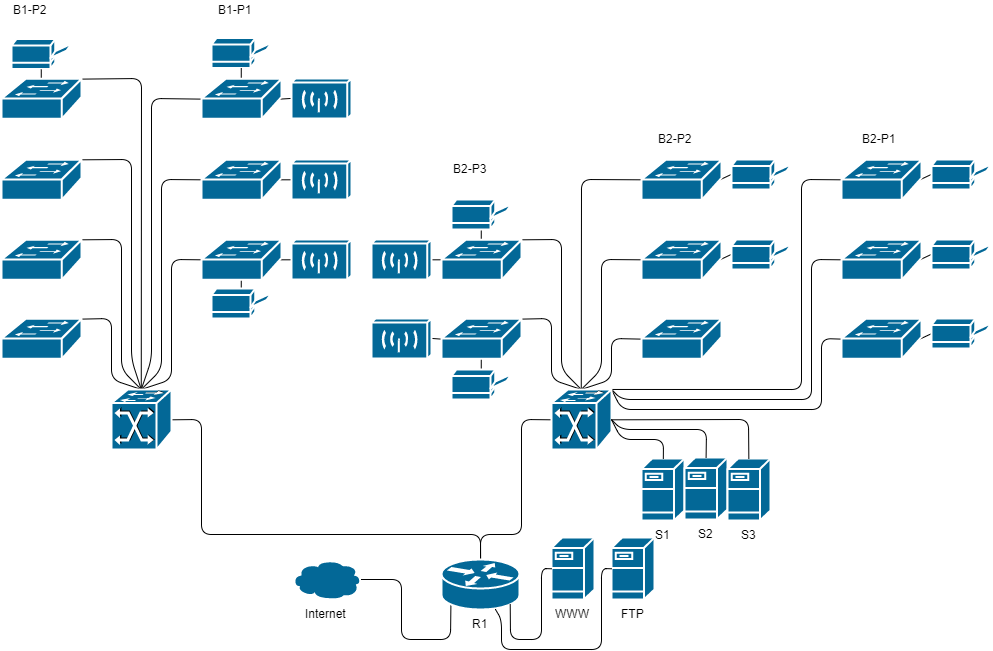
\includegraphics[scale=0.55, center]{ts2_diagram_b}
\end{center}
\newpage
\subsection{Wybór urządzeń sieciowych}
\par Ze względu na wykwalifikowaną kadrę montażystów posiadających prestiżowy certyfikat Cisco Networking Academy urządzenia tej firmy zostały wybrane. Firma Cisco znana jest również z wysokiej jakości oraz dobrych warunków gwarancji.
\par Wybrany model punktu dostepowego to Cisco WAP371-E-K9.
\begin{table}[H]
	\centering
	\caption{My caption}
	\begin{tabular}{|c|c|c|c|c|c|c|}
		\hline
		\textbf{Budynek}    & \textbf{Piętro}    & \textbf{Oznaczenie}             & \textbf{Urządzenie}                        & \textbf{GE}            & \textbf{FE}             & \textbf{Rodzaj}            \\ \hline
		\multirow{8}{*}{1}  & \multirow{5}{*}{2} & SW01-B1-P2                      & Cisco 50P SLM248GT-EU                      & -                      & 48                      & \multirow{4}{*}{Switch L2} \\ \cline{3-6}
		&                    & SW02-B1-P2                      & Cisco 50P SLM248GT-EU                      & -                      & 48                      &                            \\ \cline{3-6}
		&                    & SW03-B1-P2                      & Cisco 26P SG200-26                     	& -                      & 24                      &                            \\ \cline{3-6}
		&                    & SW03-B1-P2                      & Cisco 26P SG200-26                      	& -                      & 24                      &                            \\ \cline{3-7} 
		&                    & SW04-B1-P2                      & Cisco 10P SRW2008-K9-G5                    & 8                      & 0                       & Switch L3                  \\ \cline{2-7} 
		& \multirow{3}{*}{1} & SW05-B1-P1                      & Cisco 50P SLM248GT-EU                      & -                      & 48                      & \multirow{3}{*}{Switch L2} \\ \cline{3-6}
		&                    & SW06-B1-P1                      & Cisco 50P SLM248GT-EU                      & -                      & 48                      &                            \\ \cline{3-6}
		&                    & SW07-B1-P1                      & Cisco 50P SLM248GT-EU                      & -                      & 24                      &                            \\ \hline
		\multirow{10}{*}{2} & \multirow{4}{*}{3} & SW08-B2-P3                      & Cisco 50P SLM248GT-EU                      & -                      & 48                      & \multirow{2}{*}{Switch L2} \\ \cline{3-6}
		&                    & SW09-B2-P3                      & Cisco 26P SG200-26                      	& -                      & 24                      &                            \\ \cline{3-7} 
		&                    & SW10-B2-P3                      & Cisco 20P SRW2016-K9-EU                    & 18                     & -                       & Switch L3                  \\ \cline{3-7} 
		&                    & R0                              & Cisco RV130W-E-K9-G5                       & 4                      & -                       & Router                     \\ \cline{2-7} 
		& \multirow{3}{*}{2} & SW11-B2-P2                      & Cisco 50P SLM248GT-EU                      & -                      & 48                      & \multirow{3}{*}{Switch L2} \\ \cline{3-6}
		&                    & SW12-B2-P2                      & Cisco 26P SG200-26                      	& -                      & 24                      &                            \\ \cline{3-6}
		&                    & SW13-B2-P2                      & Cisco 26P SG200-26                      	& -                      & 24                      &                            \\ \cline{2-7} 
		& \multirow{3}{*}{1} & SW14-B2-P1                      & Cisco 26P SG200-26U                      	& -                      & 24                      & \multirow{3}{*}{Switch L2} \\ \cline{3-6}
		&                    & SW15-B2-P1 						& Cisco 26P SG200-26 						& - & 24 &                            \\ \cline{3-6}
		&                    & SW16-B2-P   						& Cisco 26P SG200-26 & - & 24 &                            \\ \hline
	\end{tabular}
\end{table}

\subsection{Projekt adresacji IP}
\begin{table}[H]
	\centering
	\caption{My caption}
	\begin{tabular}{|c|c|c|c|}
		\hline
		& \textbf{Adres podsieci} & \textbf{Maska}      & \textbf{Używane adresy}     \\ \hline
		\textbf{Brama domyślna} & 192.168.0.0             & 255.255.255.0 (/24) & 192.168.0.1                 \\ \hline
		\textbf{VLAN1 (Konstruktorzy)}          & 192.168.1.0             & 255.255.255.0 (/24) & 192.168.1.1 - 192.168.1.178 \\ \hline
		\textbf{VLAN2 (Projektanci)}          & 192.168.2.0             & 255.255.255.0 (/24) & 192.168.2.1 - 192.168.2.247 \\ \hline
		\textbf{VLAN3 (Architekci)}          & 192.168.3.0             & 255.255.255.0 (/24) & 192.168.3.1 - 192.168.3.90  \\ \hline
		\textbf{VLAN4 (Zarząd)}          & 192.168.4.0             & 255.255.255.0 (/24) & 192.168.4.1 - 192.168.4.59  \\ \hline
		\textbf{Serwery}        & 192.168.5.0             & 255.255.255.0 (/24) & 192.168.5.1 - 192.168.5.3   \\ \hline
		\textbf{Drukarki}       & 192.168.6.0             & 255.255.255.0 (/24) & 192.168.6.1 - 192.168.6.11  \\ \hline
	\end{tabular}
\end{table}

\newpage
\subsection{Projekt konfiguracji urządzeń}
\begin{table}[H]
	\centering
	\caption{My caption}
	\begin{tabular}{|c|c|c|c|c|}
		\hline
		\multicolumn{5}{|c|}{\textbf{Router}}                                                                  \\ \hline
		\textbf{Urządzenie}      & \textbf{Port}  & \textbf{Adres sieci} & \textbf{Maska}     & \textbf{Adres} \\ \hline
		\textbf{Serwer FTP}      & interface g0/0 & 45.0.0.0             & 255.255.0.0 (/16)  & 45.0.1.1       \\ \hline
		\textbf{Sieć wewnętrzna} & interface g0/1 & 192.168.0.0          & 255.255.255.0(/24) & 192.168.0.2    \\ \hline
		\textbf{Serwer WWW}      & interface g0/2 & 46.0.0.0             & 255.255.0.0 (/16)  & 46.0.1.1       \\ \hline
		\textbf{Internet}        & interface g0/3 & 47.0.0.0             & 255.255.0.0 (/16)  & 47.0.1.1       \\ \hline
	\end{tabular}
\end{table}

\begin{table}[H]
	\centering
	\caption{My caption}
	\begin{tabular}{cccc}
		\hline
		\multicolumn{1}{|c|}{\textbf{VLAN1}}                 & \multicolumn{1}{c|}{\multirow{2}{*}{192.168.1.0}} & \multicolumn{1}{c|}{255.255.255.0 (/24)}     & \multicolumn{1}{c|}{192.168.1.1 - 192.168.1.178} \\ \cline{1-1} \cline{3-4} 
		\multicolumn{1}{|c|}{\textbf{interface vlan1}}       & \multicolumn{1}{c|}{}                             & \multicolumn{1}{c|}{255.255.255.0 (/24)}     & \multicolumn{1}{c|}{192.168.1.254}               \\ \hline
		&                                                   &                                              &                                                  \\ \hline
		\multicolumn{1}{|c|}{\textbf{VLAN2}}                 & \multicolumn{1}{c|}{\multirow{2}{*}{192.168.2.0}} & \multicolumn{1}{c|}{255.255.255.0 (/24)}     & \multicolumn{1}{c|}{192.168.2.1 - 192.168.2.247} \\ \cline{1-1} \cline{3-4} 
		\multicolumn{1}{|c|}{\textbf{interface vlan2}}       & \multicolumn{1}{c|}{}                             & \multicolumn{1}{c|}{255.255.255.0 (/24)}     & \multicolumn{1}{c|}{192.168.2.254}               \\ \hline
		&                                                   &                                              &                                                  \\ \hline
		\multicolumn{1}{|c|}{\textbf{VLAN3}}                 & \multicolumn{1}{c|}{\multirow{2}{*}{192.168.3.0}} & \multicolumn{1}{c|}{255.255.255.0 (/24)}     & \multicolumn{1}{c|}{192.168.3.1 - 192.168.3.90}  \\ \cline{1-1} \cline{3-4} 
		\multicolumn{1}{|c|}{\textbf{interface vlan3}}       & \multicolumn{1}{c|}{}                             & \multicolumn{1}{c|}{255.255.255.0 (/24)}     & \multicolumn{1}{c|}{192.168.3.254}               \\ \hline
		&                                                   &                                              &                                                  \\ \hline
		\multicolumn{1}{|c|}{\textbf{VLAN4}}                 & \multicolumn{1}{c|}{\multirow{2}{*}{192.168.4.0}} & \multicolumn{1}{c|}{255.255.255.0 (/24)}     & \multicolumn{1}{c|}{192.168.4.1 - 192.168.4.59}  \\ \cline{1-1} \cline{3-4} 
		\multicolumn{1}{|c|}{\textbf{interface vlan4}}       & \multicolumn{1}{c|}{}                             & \multicolumn{1}{c|}{255.255.255.0 (/24)}     & \multicolumn{1}{c|}{192.168.4.254}               \\ \hline
		&                                                   &                                              &                                                  \\ \hline
		\multicolumn{1}{|c|}{\textbf{VLAN5 (serwery wewn.)}} & \multicolumn{1}{c|}{\multirow{2}{*}{192.168.5.0}} & \multicolumn{1}{c|}{255.255.255.0 (/24)}     & \multicolumn{1}{c|}{192.168.5.1 - 192.168.5.3}   \\ \cline{1-1} \cline{3-4} 
		\multicolumn{1}{|c|}{\textbf{interflace vlan5}}      & \multicolumn{1}{c|}{}                             & \multicolumn{1}{c|}{255.255.255.0 (/24)}     & \multicolumn{1}{c|}{192.168.5.254}               \\ \hline
		&                                                   &                                              &                                                  \\ \hline
		\multicolumn{1}{|c|}{\textbf{VLAN6 (drukarki)}}      & \multicolumn{1}{c|}{\multirow{2}{*}{192.168.6.0}} & \multicolumn{1}{c|}{255.255.255.0 (/24)}     & \multicolumn{1}{c|}{192.168.6.1 - 192.168.6.11}  \\ \cline{1-1} \cline{3-4} 
		\multicolumn{1}{|c|}{\textbf{interface vlan6}}       & \multicolumn{1}{c|}{}                             & \multicolumn{1}{c|}{255.255.255.0 (/24)}     & \multicolumn{1}{c|}{192.168.6.254}               \\ \hline
		&                                                   &                                              &                                                  \\ \hline
		\multicolumn{1}{|c|}{\textbf{Urządzenie}}            & \multicolumn{1}{c|}{\textbf{Adres}}               & \multicolumn{1}{c|}{\textbf{Maska podsieci}} & \multicolumn{1}{c|}{\textbf{Brama domyślna}}     \\ \hline
		\multicolumn{1}{|c|}{\textbf{Serwer FTP}}            & \multicolumn{1}{c|}{45.0.1.2}                     & \multicolumn{1}{c|}{255.255.0.0 (/16)}       & \multicolumn{1}{c|}{45.0.1.1}                    \\ \hline
		\multicolumn{1}{|c|}{\textbf{Serwer WWW}}            & \multicolumn{1}{c|}{46.0.1.2}                     & \multicolumn{1}{c|}{255.255.0.0 (/16)}       & \multicolumn{1}{c|}{46.0.1.1}                    \\ \hline
		\multicolumn{1}{|c|}{\textbf{S1}}                    & \multicolumn{1}{c|}{192.168.5.1}                  & \multicolumn{1}{c|}{255.255.255.0 (/24)}     & \multicolumn{1}{c|}{192.168.5.254}               \\ \hline
		\multicolumn{1}{|c|}{\textbf{S2}}                    & \multicolumn{1}{c|}{192.168.5.2}                  & \multicolumn{1}{c|}{255.255.255.0 (/24)}     & \multicolumn{1}{c|}{192.168.5.254}               \\ \hline
		\multicolumn{1}{|c|}{\textbf{S3}}                    & \multicolumn{1}{c|}{192.168.5.3}             \textsl{}     & \multicolumn{1}{c|}{255.255.255.0 (/24)}     & \multicolumn{1}{c|}{192.168.5.254}               \\ \hline
	\end{tabular}
\end{table}

\newpage
\subsection{Projekt podłączenia do Internetu}

\newpage
\subsection{Analiza bezpieczeństwa i niezawodności sieci}
\subsubsection{Ochrona przed wirusami}
\par Jak wiadomo pracownicy mogą być ofiaramy przeróżnych ataków, niekoniecznie przez internet. Źródłem zagrożenia może być chociażby pendrive z wirusem. Aby ustrzec
firmę przed działaniem niechcianego oprogramowania, zdecydowaliśmy się na zakup licencji antywirusa F-Secure. Możliwości finansowe firmy pozwalają na zakup takiej licencji, 
a według badań przeprowadzonych przez niezależne ośrodki badawcze program radzi sobie bardzo dobrze z większością zagrożeń. Jest on również małym obciążeniem dla procesora,
a jego częste aktualizacje powodują zwiększenie skutecznośći ochrony.
\subsubsection{Internet}
\par Router łączący sieć z internetem posiada wbudowany firewall, aby chronić sieć wewnętrzną przed atakami z zewnątrz. W dodatku program antywirusowy F-Secure posiada opcje firewalla oraz skanowania przychodzących maili. Potrafi on ostrzec przed zagrożeniem znajdującym się w załączniku, lub w linku przesłanym w wiadomości. W ten sposób nawet przy dużej nieuwadze pracownik asystem nie jest od razu narażony na atak.
\subsubsection{Awaria zasilania}
\par W razie awarii zasilania serwery zaopatrzone są w UPS-y oraz w planach jest zakup własnego agregatu prądotwórczego. W takiej sytuacji firma jest w stanie pracować bez problemów
przez pewien okres czasu aż do naprawy zasilania.

\subsection{Kosztorys}

%----------------------------------------------------------------------------------------
%	SECTION 6
%----------------------------------------------------------------------------------------
\newpage
\section{Karty katalogowe proponowanych urządzeń}

%----------------------------------------------------------------------------------------
%	BIBLIOGRAPHY
%----------------------------------------------------------------------------------------
%\newpage
%\bibliographystyle{apalike}
%\begin{thebibliography}{9}
%
%\bibitem{wikipediacluster} 
%Wikipedia: Computer cluster,
%\\\texttt{https://en.wikipedia.org/wiki/Computer\_cluster}
%	
%\bibitem{wikipediasieve} 
%Wikipedia: Sieve of Erastosthenes,
%\\\texttt{https://en.wikipedia.org/wiki/Sieve\_of\_Eratosthenes}
%
%\end{thebibliography}

%----------------------------------------------------------------------------------------
\end{document}